\begin{figure}
	\begin{tikzpicture}
	\sbEntree{E}
	\sbComp{a}{E}
	\sbBloc{b}{P}{a}
	\sbRelier[$x_{d}$]{E}{a}
	\sbComp{c}{b}	
	\sbRelier[$\epsilon_x$]{a}{b}
	\sbRelier[$\dot{x}_{d}$]{b}{c}
	
	\sbBloc{d}{PI}{c}	
	\sbRelier[$\epsilon_{\dot{x}}$]{c}{d}
	
	\sbComp{e}{d}	
	\sbRelier[$I_d$]{d}{e}
	
	\sbBloc{f}{PI}{e}	
	\sbRelier[$\epsilon_{I}$]{e}{f}
	
	
	\sbBloc{g}{Process}{f}	
	\sbRelier{f}{g}
	
	
	\sbSortie{h}{g}
	\sbRelier{g}{h}
	
	\sbRenvoi{g}{a}{$x_a$}
	\sbRenvoi{g}{c}{$\dot{x}_a$}
	\sbRenvoi{g}{e}{$I_a$}
	
	\draw [color=gray,thick](0,-2) rectangle (4.4,1.5);
	\node at (0.5,1) [below=10mm, right=0mm] {sbRIO FPGA};
	
		\draw [color=gray,thick](4.4,-2) rectangle (10.75,1.5);
		\node at (6.5,1) [below=10mm, right=0mm] {ESCON controller};
	
	\end{tikzpicture}
	\caption{Embedded cascade control. x is position, $\dot{x}$ is speed, I is current. d index means demand, a index means actual value.}
\end{figure}

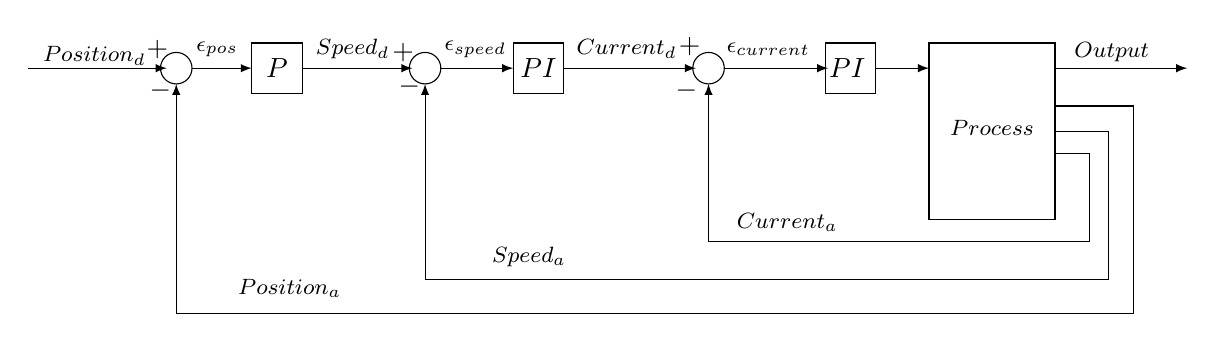
\begin{tikzpicture}[scale=0.8]

\draw [-latex] (1.25,3.4) ellipse (0.25 and 0.25);
\node at (-1.45,3.4) {\normalsize{$PI$}};
\node at (3.45,3.4) {\normalsize{$PI$}};
\node at (7.65,3.65) {\normalsize{\footnotesize$Output$}};
\node at (5.75,2.45) {\normalsize{\footnotesize$Process$}};
\draw [-latex] (-1.85,3.8) rectangle (-1.05,3);
\draw [-latex] (3.1,3.8) rectangle (3.9,3);
\draw [-latex](-1.05,3.4) -- (1.05,3.4);
\draw [-latex] (-3.25,3.4) ellipse (0.25 and 0.25);
\draw [-latex](-3,3.4) -- (-1.85,3.4);
\node at (-2.45,3.7) {\footnotesize$\epsilon_{speed}$};
\node at (2.2,3.7) {\footnotesize$\epsilon_{current}$};
\node at (-5.6,3.4) {\normalsize{$P$}};
\draw [-latex] (-6,3.8) rectangle (-5.2,3);
\draw [-latex](-5.2,3.4) -- (-3.45,3.4);

\draw [-latex](1.5,3.4) -- (3.15,3.4);
\draw [-latex](3.9,3.4) -- (4.75,3.4);
\draw [-latex](6.75,3.4) -- (8.85,3.4);

\draw [-latex](6.75,2.05) -- (7.3,2.05) -- (7.3,0.65)-- (1.25,0.65)-- (1.25,3.15);
\draw [-latex](6.75,2.4) -- (7.6,2.4) -- (7.6,0.05)-- (-3.25,0.05)-- (-3.25,3.15);
\draw [-latex](6.75,2.8) -- (8,2.8) -- (8,-0.5)-- (-7.2,-0.5)-- (-7.2,3.15);

\node at (0.95,3.75) {$+$};
\node at (0.9,3.05) {$-$};

\draw [-latex] (-7.2,3.4) ellipse (0.25 and 0.25);
\draw [-latex](-6.95,3.4) -- (-6,3.4);
\node at (-3.5,3.1) {$-$};

\draw [-latex](-9.55,3.4) -- (-7.35,3.4);
\node at (-8.5,3.6) {\footnotesize$Position_d$};
\node at (-7.45,3.05) {$-$};
\node at (-6.55,3.7) {\footnotesize$\epsilon_{pos}$};
\node at (-4.4,3.7) {\footnotesize$Speed_d$};
\node at (-0.05,3.7) {\footnotesize$Current_d$};
\node at (2.5,0.95) {\footnotesize$Current_a$};
\node at (-1.6,0.4) {\footnotesize$Speed_a$};
\node at (-5.4,-0.1) {\footnotesize$Position_a$};


\node (v2) at (-7.5,3.7) {$+$};
\node (v2) at (-3.6,3.65) {$+$};
\draw  (4.75,3.8) rectangle (6.75,1);
\end{tikzpicture}
	